%\input{secao1}
\section{Desenvolvimento do Projeto}

No período de abril até maio, os alunos desenvolveram a interface geral do site e um jogo de reflexo utilizando HTML, CSS e JavaScript. Durante esse período, foram implementadas interfaces gráficas, estilização visual, lógica de programação e sistemas de interação entre jogadores.

\subsection{Interface do Site}

A interface principal do site foi criada utilizando HTML e CSS, permitindo a organização dos jogos desenvolvidos pelo grupo em uma estrutura simples e intuitiva.

\begin{figure}[h]
    \centering
    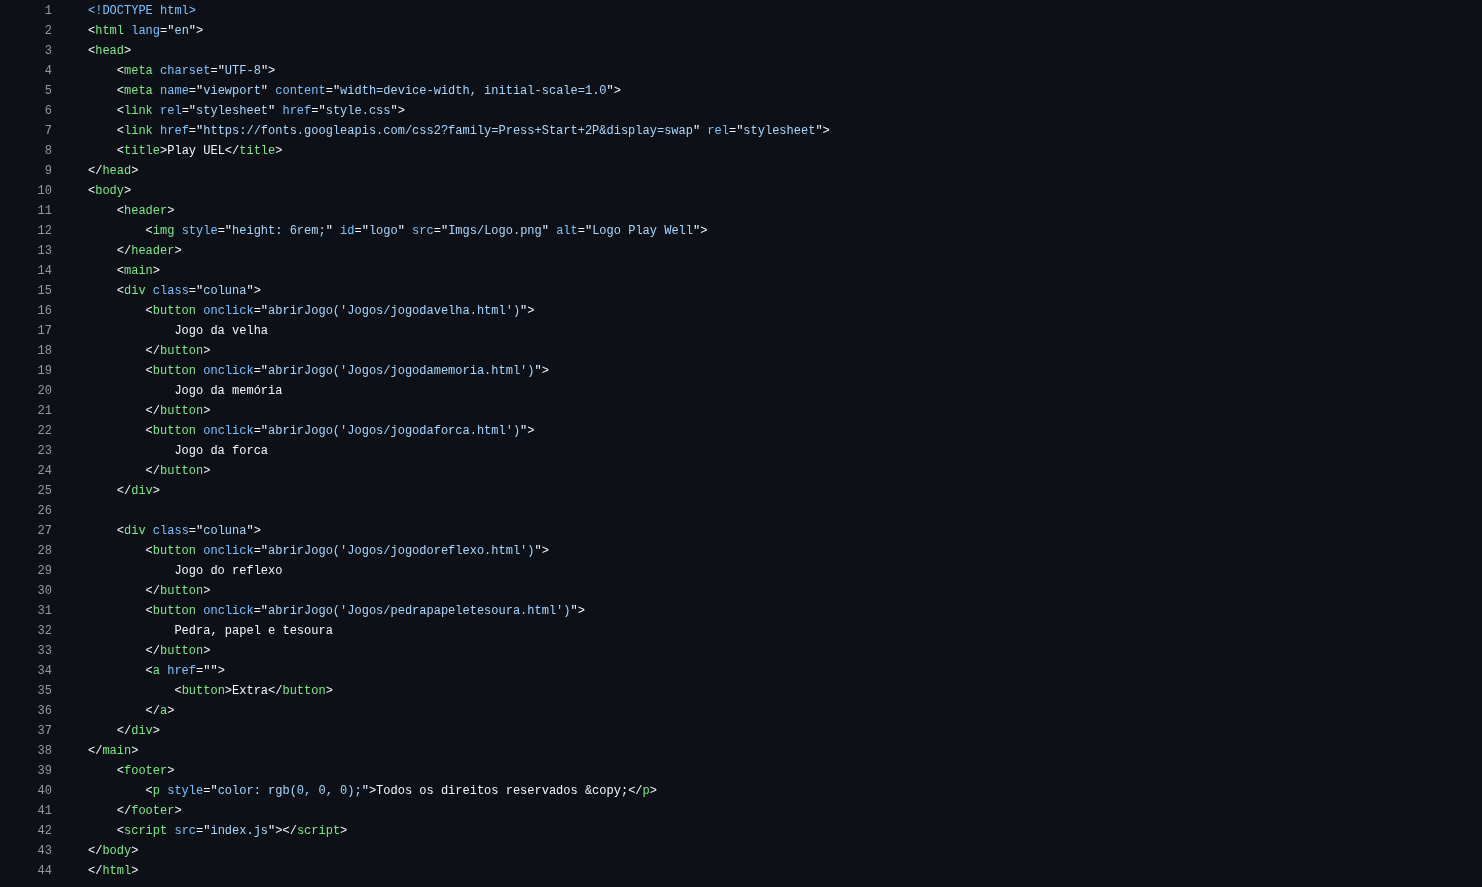
\includegraphics[width=0.75\textwidth]{imgs/HTMLinterface.png}
    \caption{Estrutura HTML da interface principal do site.}
\end{figure}

\begin{figure}[h]
    \centering
    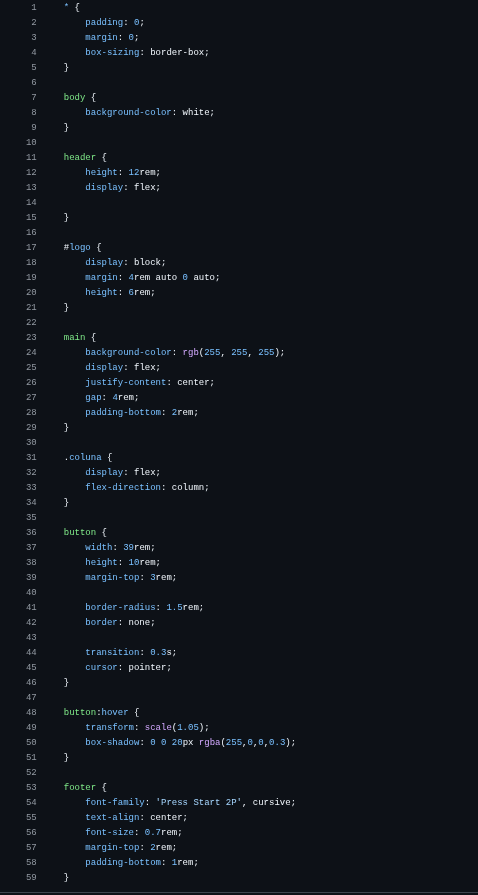
\includegraphics[width=0.75\textwidth]{imgs/CSSinterface.png}
    \caption{Estilização da interface principal utilizando CSS.}
\end{figure}

\begin{figure}[h]
    \centering
    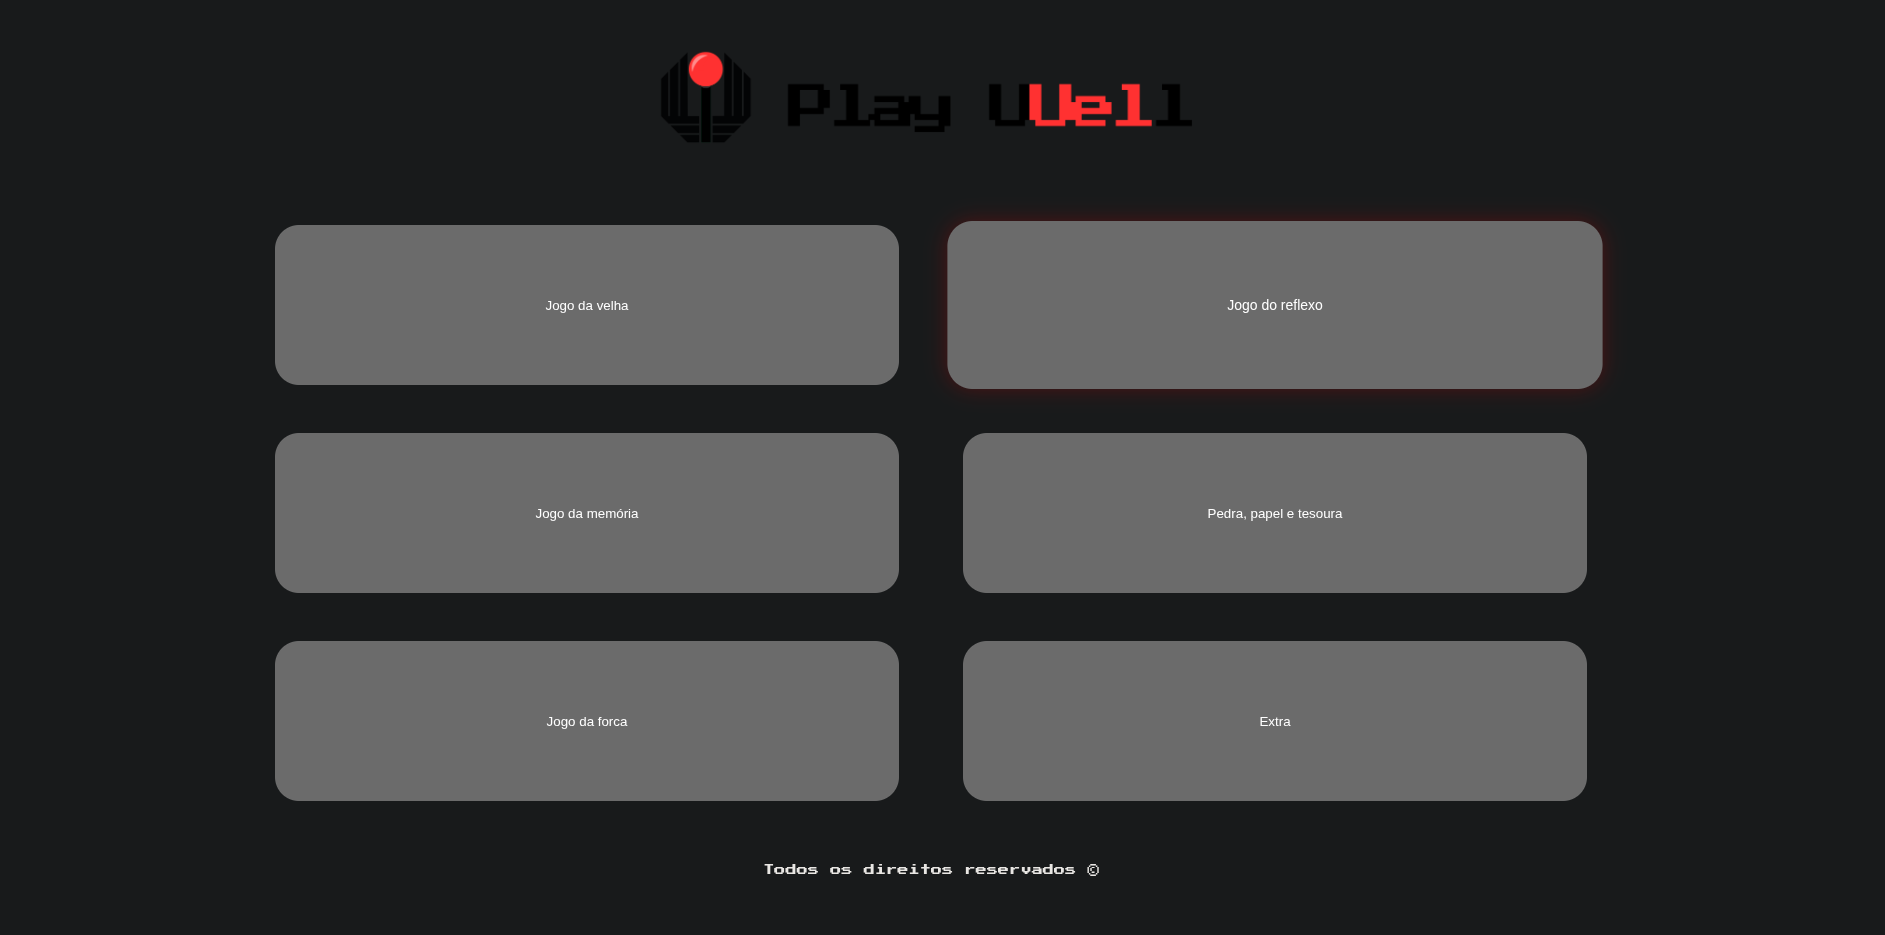
\includegraphics[width=0.75\textwidth]{imgs/InterfaceSite.png}
    \caption{Resultado visual da interface principal do site.}
\end{figure}

\clearpage

\subsection{Desenvolvimento do Jogo Duelo de Reflexo}

O jogo Duelo de Reflexo foi desenvolvido utilizando JavaScript para controle da lógica de jogo, HTML para estruturação da página e CSS para estilização visual e animações.

\begin{figure}[h]
    \centering
    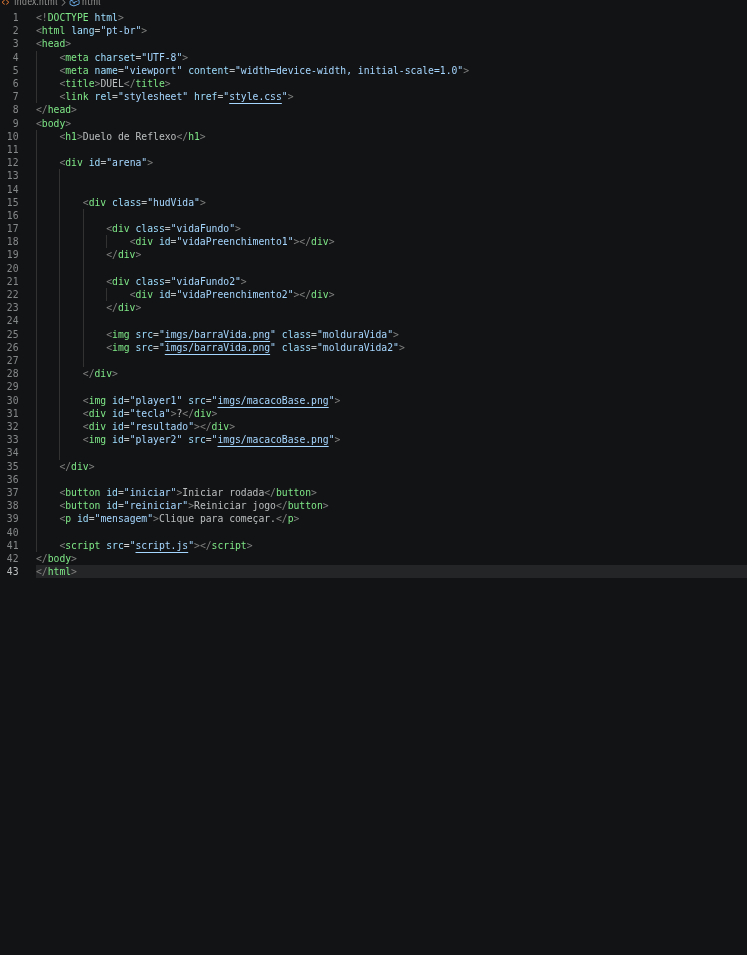
\includegraphics[width=0.75\textwidth]{imgs/HtmlReflexo.png}
    \caption{Estrutura HTML da página do jogo Duelo de Reflexo.}
\end{figure}

\begin{figure}[h]
    \centering
    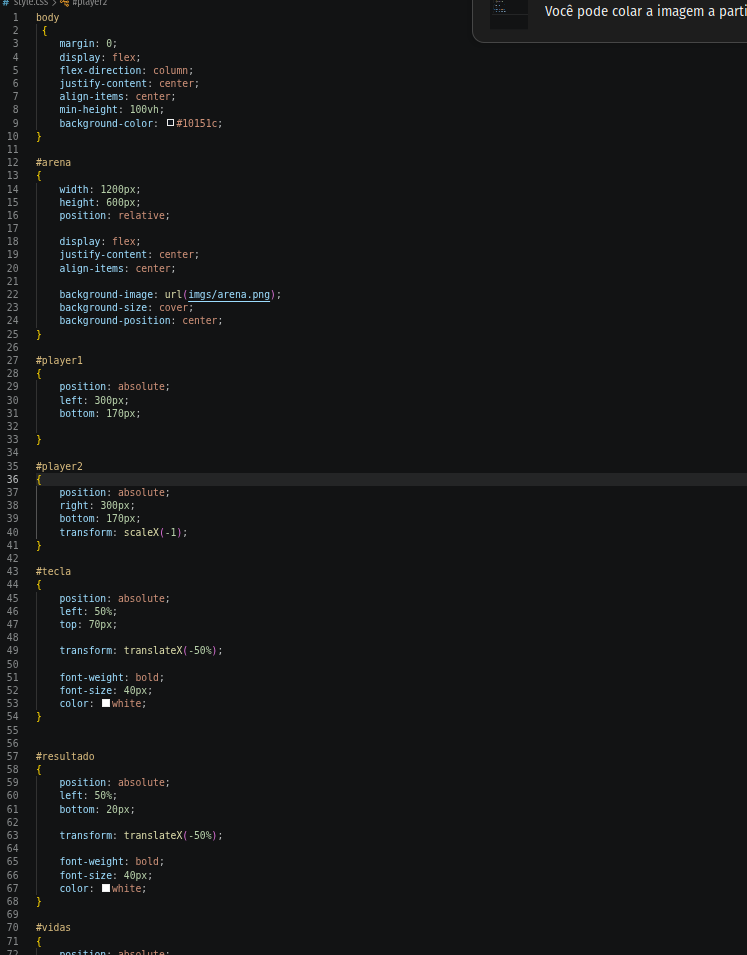
\includegraphics[width=0.75\textwidth]{imgs/ReflexoCss1.png}
    \caption{Trecho da estilização visual do jogo utilizando CSS.}
\end{figure}

\begin{figure}[h]
    \centering
    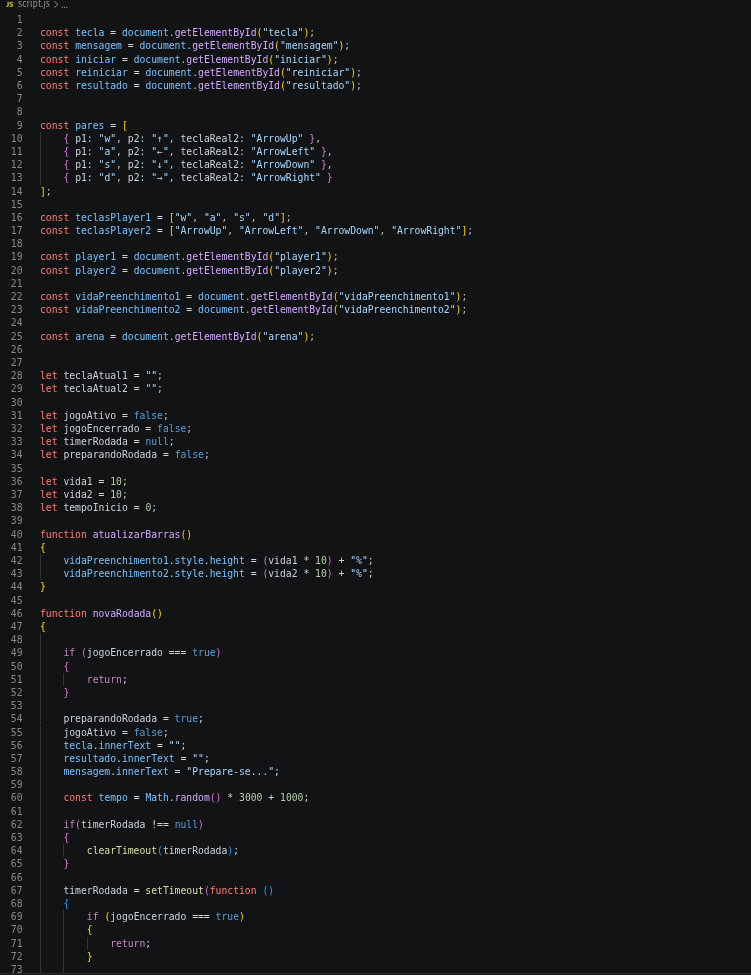
\includegraphics[width=0.75\textwidth]{imgs/ReflexoJs1.png}
    \caption{Trecho da lógica implementada em JavaScript para o jogo.}
\end{figure}

\begin{figure}[h]
    \centering
    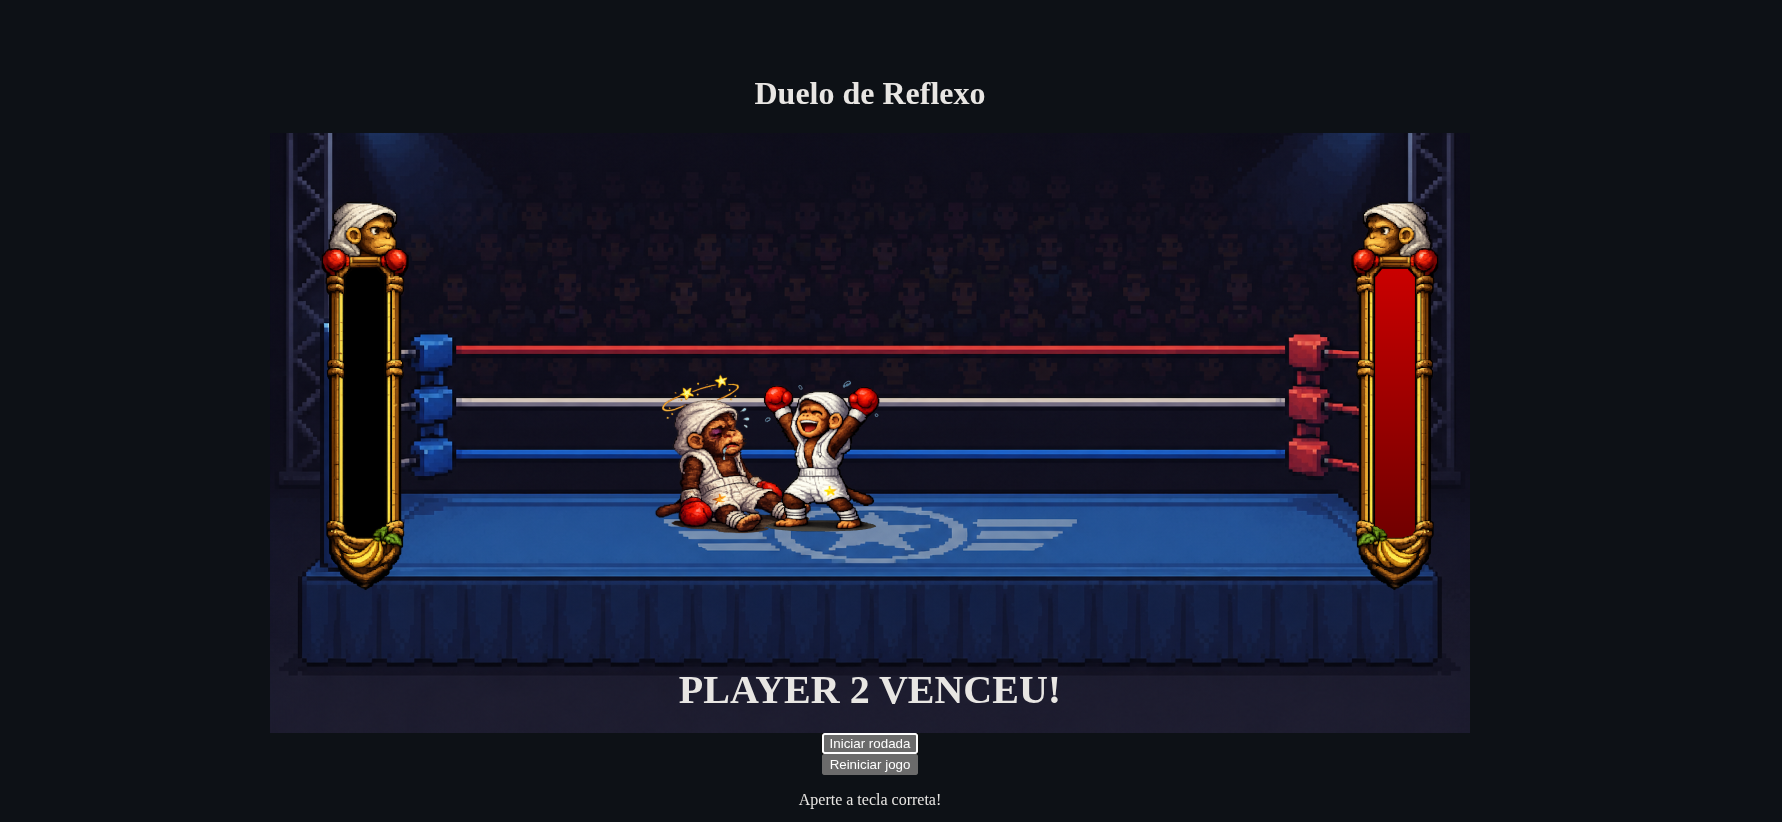
\includegraphics[width=0.75\textwidth]{imgs/jogoReflexo.png}
    \caption{Tela do jogo Duelo de Reflexo em funcionamento.}
\end{figure}
%\input{secao2}